%!TEX encoding = UTF-8 Unicode 

\newif\ifen\entrue
% Language selector; must be on line 3
% Change to false to export Korean

\documentclass[11pt,mathserif,notheorems]{beamer}
\usetheme{CambridgeUS}
\usepackage[parfill]{parskip}
\usepackage{layout}
\usepackage{color}
\usepackage{amsmath,amssymb}
\usepackage{amsthm}
\usepackage{graphicx}
\usepackage{relsize}
\usepackage{kotex}
\usepackage{diagbox}
\usepackage{multirow}
\usepackage{hyperref}
\hyperbaseurl{}
\urlstyle{same}
\usepackage[ruled]{algorithm2e}
\newcommand{\lIfElse}[3]{\lIf{#1}{#2 \textbf{else}~#3}}
%\usepackage{bbold}
%\usepackage{kbordermatrix}
\usepackage{xcolor}
%\usepackage{cutwin}
\usepackage{tabularx}
%\usepackage{pgfplots}
%\usepgfplotslibrary{external} % Prevents memory overflow issues w pgfplots
%\tikzexternalize
%\setlength{\jot}{0pt}


\usepackage{stackengine}
\newcommand\xrowht[2][0]{\addstackgap[.5\dimexpr#2\relax]{\vphantom{#1}}}



\ifen
{
\newtheorem{theorem}{Theorem}
\newtheorem{lemma}{Lemma}
\newtheorem{corollary}{Corollary}
\newtheorem{conjecture}{Conjecture}
\theoremstyle{definition}
\newtheorem{definition}{Definition}
\newtheorem{assumption}{Assumption}
\newtheorem{proposition}{Proposition}
\newtheorem{example}{Example}
\newtheorem{problem}{Problem}
}
\else {
\newtheorem{theorem}{정리}
\newtheorem{lemma}{기본정리}
\newtheorem{corollary}{따름정리}
\newtheorem{conjecture}{추측}
\theoremstyle{definition}
\newtheorem{definition}{정의}
\newtheorem{assumption}{가정}
\newtheorem{proposition}{제의}
\newtheorem{example}{예}
\newtheorem{problem}{문제}
}
\fi

\ifen \else \renewcommand{\proofname}{증명\@} \fi

\DeclareMathOperator*{\argmin}{arg\,min}
\DeclareMathOperator*{\argmax}{arg\,max}
\DeclareMathOperator*{\expd}{exp.}
\DeclareMathOperator*{\BR}{BR}

\newcommand*{\vertbar}{\rule[-1ex]{0.5pt}{2.5ex}}
\newcommand*{\horzbar}{\rule[.5ex]{2.5ex}{0.5pt}}
\setcounter{MaxMatrixCols}{20}

\DeclareGraphicsExtensions{.pdf,.png,.jpg}
\def\pfbox{\,\lower0.9pt\vbox{\hrule \hbox{\vrule height 0.2
cm \hskip 0.2 cm \vrule height 0.2 cm}\hrule}\,}
\newcommand{\nimplies}{%
  \mathrel{{\ooalign{\hidewidth$\not\phantom{=}$\hidewidth\cr$\implies$}}}}






\ifen 
\title{The College Application Problem}
\author{Max Kapur}
\institute{Seoul National University\\
Department of Industrial Engineering \\
Management Science/Optimization Lab\\
\url{maxkapur@snu.ac.kr}\\}
\date{May 13, 2022}
\else
\title[대학 지원 최적화 문제]{대학 지원 최적화 문제}
\author{Max Kapur}
\institute{서울대학교 산업공학과 \\
경영과학/최적화 연구실\\
\url{maxkapur@snu.ac.kr}\\
\vspace{0.5em}
지도 교수: 홍성필}
\date[2022년 5월 13일]{2022년 5월 13일\\석사논문합동발표회}
\fi


\beamertemplatenavigationsymbolsempty

\definecolor{teal}{HTML}{008080}
\definecolor{olivedrab}{HTML}{6b8e23}
\definecolor{crimson}{HTML}{b22222}
\definecolor{palettetertiary}{HTML}{4169E1}
\definecolor{beige}{HTML}{f5fffa}
\definecolor{azure}{HTML}{F5F5F5}
\definecolor{rebeccapurple}{HTML}{663399}

% Corrects color spacing issue in math mode
\makeatletter
\renewcommand*{\@textcolor}[3]{%
  \protect\leavevmode
  \begingroup
    \color#1{#2}#3%
  \endgroup
}
\makeatother


\setbeamercolor{normal text}{fg=black,bg=white}
\setbeamercolor{alerted text}{fg=red}
\setbeamercolor{example text}{fg=black}

\setbeamercolor{palette primary}{fg=black, bg=beige}
%%\setbeamercolor{palette secondary}{fg=black, bg=beige}
\setbeamercolor{palette tertiary}{fg=white, bg=palettetertiary}

\setbeamercolor{frametitle}{fg=black, bg=azure}
\setbeamercolor{title}{fg=black, bg=azure}

\setbeamertemplate{items}[square]
\setbeamercolor*{item}{fg=palettetertiary}
%\beamertemplateshadingbackground{white}{white}
%\setbeamertemplate{caption}[numbered]
\setbeamertemplate{headline}{}



 \setbeamertemplate{caption}[numbered]
\setbeamertemplate{footline} {
  \leavevmode%
  \hbox{%
  \begin{beamercolorbox}[wd=.25\paperwidth,ht=2.65ex,dp=1.2ex,left]{author in head/foot}%
  \hspace*{1.5ex}\insertshortauthor
  \end{beamercolorbox}%
  \begin{beamercolorbox}[wd=.27\paperwidth,ht=2.65ex,dp=1.2ex,left]{date in head/foot}%
  \hspace*{1ex}
    \ifnum \theframenumber=1{}
    \else \insertshorttitle%~\textbar~\insertsectionhead
    \fi
     \end{beamercolorbox}%
  \begin{beamercolorbox}[wd=.23\paperwidth,ht=2.65ex,dp=1.2ex,right]{date in head/foot}%
    \ifnum \theframenumber=1{}
    \else \insertsectionhead
    \fi
  \hspace*{2ex}
     \end{beamercolorbox}%
       \begin{beamercolorbox}[wd=.15\paperwidth,ht=2.65ex,dp=1.2ex,left]{author in head/foot}%
  \hspace*{1.5ex}\insertshortdate
  \end{beamercolorbox}%
  \begin{beamercolorbox}[wd=.1\paperwidth,ht=2.65ex,dp=1.2ex,right]{author in head/foot}%
    \insertframenumber{} / \inserttotalframenumber
    \hspace*{1.5ex}
  \end{beamercolorbox}
}%
  \vskip0pt%
}

\overfullrule=0pt
\newcounter{usec}[section]

\makeatletter
\newcommand{\rmnum}[1]{\romannumeral #1}
\newcommand{\Rmnum}[1]{\expandafter\@slowromancap\romannumeral #1@}
\makeatother
\setbeamertemplate{theorems}[numbered]





\begin{document}


\begin{frame}
\titlepage
\end{frame}





\ifen \section{Introduction} \else \section{서론} \fi







\ifen {
\begin{frame}{Introduction}
The optimal college application problem is a \textbf{novel combinatorial optimization problem}.

It involves \textbf{maximizing the expected maximum} of a portfolio of random variables subject to a budget constraint.

Methodological orientation:
\begin{itemize}
\item Investment with uncertain payoff, search for the efficient frontier recall \textbf{portfolio allocation} models. 
\item Generalizes the \textbf{knapsack problem}: Integral packing constraint, NP-completeness, approximation algorithms.
\item Objective is a \textbf{submodular set function}.
\end{itemize}

Today's presentation: \textbf{define the problem} and briefly summarize our \textbf{solution algorithms}. 
\end{frame}
} \else {
\begin{frame}{서론}
대학 지원 최적화 문제는 \textbf{새로운 조합 최적화 문제}이다.

예산 제약 조건 하에서, 다수 확률 변수로 이뤄진 포트폴리오의 \textbf{기대 최댓값을 최대화}하는 문제이다.

방법론적 지향:
\begin{itemize}
\item 불확실한 성과, 효율적 투자선이 존재하므로 \textbf{일종의 포트폴리오 배분} 모형. 
\item \textbf{배낭 문제의 일반화}: 정수 채우기 (packing) 제약식, NP-completeness, 근사 해법의 필요.
\item 목적함수는 \textbf{submodular 집합 함수}.
\end{itemize}

\mbox{오늘 발표에서는 \textbf{문제를 정의하고 본 연구가 제시하는 해법}을 요약한다.}
\end{frame}
} \fi











\ifen \section{Model} \else \section{모형} \fi



\ifen {
\begin{frame}{The admissions process}
Consider a \textbf{single student's} college application decision.

Market contains $m$ \textbf{schools}, indexed by $\mathcal{C} = \{ 1\dots m\}$. School $j$ is named $c_j$.

We know the student's \textbf{admissions probability} $f_j$ at each school.

Let the independent \textbf{random variable} $Z_j \sim \operatorname{Bernoulli}(f_j) = 1$ if student is admitted, $0$ otherwise. 

Let $\mathcal{X} \subseteq \mathcal{C}$ denote the set of schools, or \textbf{application portfolio}, to which a student applies.

Application fees, time to write essays, and/or legal limits \textbf{constrain} applicant behavior. We consider a single knapsack constraint $\sum_{j\in \mathcal{X}} g_j \leq H$ where $g_j$ is called $c_j$'s \textbf{application cost}. 
\end{frame}
} \else {
\begin{frame}{입학 과정}
\textbf{단 한 명의 학생}의 의사결정에 집중하자.

시장은 $m$개의 \textbf{대학교}를 포함하며, 그의 지표 집합은 $\mathcal{C} = \{ 1\dots m\}$. $j$번째 학교의 이름은 $c_j$.

각 학교에 대해 학생의 \textbf{합격 확률} $f_j$가 주어져 있다.

\looseness=-1
독립 \textbf{확률 변수} $Z_j \sim \operatorname{Bernoulli}(f_j)$는 학생이 합격하면 $1$, 아니면 $0$.

\looseness=-1
학생이 지원하는 학교의 집합 $\mathcal{X} \subseteq \mathcal{C}$를 \textbf{지원 포트폴리오}라고 부른다.

지원 전형료 예산, 원서를 작성하는 시간, 또는 나라의 정책에 따라 \textbf{지원 행동이 제한된다}. 본 논문은 단일 배낭 제약식 $\sum_{j\in \mathcal{X}} g_j \leq H$를 고려하며, 이때 $g_j$는 $c_j$의 \textbf{지원 비용}이라고 부른다. 
\end{frame}
} \fi
















\ifen {
\begin{frame}{Utility model}
Let $t_j \geq 0$ denote the \textbf{utility} the student receives if she attends $c_j$. Wlog, $t_j \leq t_{j+1}$.

Let $t_0$ denote her utility if she doesn't get into college. Wlog, $t_0 =0$ (see paper).

The student's overall utility is the $t_j$-value associated with the \textbf{best} school she applies to and gets into:
\[\text{Utility} =\max\bigr\{t_0, \max\{t_j Z_j : j \in \mathcal{X}\}\bigr\}\]
The expected value of this quantity is called the \textbf{valuation} $v(\mathcal{X})$ of the portfolio $\mathcal{X}$. 
\end{frame}
} \else {
\begin{frame}{효용 모형}
$c_j$에 다니면 $t_j \geq 0$ 단위의 \textbf{효용}이 발생한다. Wlog, $t_j \leq t_{j+1}$.

어떤 대학에도 합격하지 않았을 때 효용은 $t_0$이며, wlog $t_0 =0$임을 가정할 수 있다 (논문에서 증명).

학생의 총 효용은 그가 지원하고 합격하는 \textbf{가장 좋은} 학교의 $t_j$-값:
\[\text{효용} =\max\bigr\{t_0, \max\{t_j Z_j : j \in \mathcal{X}\}\bigr\}\]
이의 기댓값은 $\mathcal{X}$의 \textbf{가치}라고 부르며 $v(\mathcal{X})$처럼 표기한다.
\end{frame}
} \fi



\ifen {
\begin{frame}{Unpacking the portfolio valuation function}
To get $v(\mathcal{X})$ into a tractable form, let $p_j(\mathcal{X})$ denote the probability that the student \textbf{attends} $c_j$.

This happens if and only if she \textbf{applies} to $c_j$, is \textbf{admitted} to $c_j$, and is \textbf{not admitted} to any school she prefers to $c_j$:
\begin{align*}
p_j(\mathcal{X}) &= 
\begin{cases}
\displaystyle f_j  \prod_{\substack{i \in \mathcal{X}: \\ i > j}} (1 - f_{i}), \quad & j \in \{0\}\cup\mathcal{X}\\
0, \quad & \text{otherwise.}
\end{cases} 
\end{align*}
Therefore, 
\begin{align*}
v(\mathcal{X})
%&= \operatorname{E}\Bigl[\max\bigr\{t_0, \max\{t_j Z_j : j \in \mathcal{X}\}\bigr\}\Bigr] \\
&= \sum_{j=1}^m t_j p_j(\mathcal{X}) = \sum_{j\in \mathcal{X}} \Bigl( f_j t_j \prod_{\substack{i \in \mathcal{X}: \\ i > j}} (1 - f_{i}) \Bigr).  \label{closedformportfoliovaluationX}
\end{align*}

\end{frame}
} \else {
\begin{frame}{포트폴리오 가치의 함수 형태}
$v(\mathcal{X})$를 함수로 표현하기 위해, 학생이 $c_j$에 \textbf{진학하는} 확률을 $p_j(\mathcal{X})$라고 하자.

$c_j$에 진학하는 조건은 $c_j$에 \textbf{지원}하고, \textbf{합격}하고, $c_j$보다 선호하는 학교에는 \textbf{합격하지 않았을} 때이다.
\begin{align*}
p_j(\mathcal{X}) &= 
\begin{cases}
\displaystyle f_j  \prod_{\substack{i \in \mathcal{X}: \\ i > j}} (1 - f_{i}), \quad & j \in \{0\}\cup\mathcal{X}\\
0, \quad & \text{그렇지 않은 경우.}
\end{cases} 
\end{align*}
따라서,
\begin{align*}
v(\mathcal{X})
%&= \operatorname{E}\Bigl[\max\bigr\{t_0, \max\{t_j Z_j : j \in \mathcal{X}\}\bigr\}\Bigr] \\
&= \sum_{j=1}^m t_j p_j(\mathcal{X}) = \sum_{j\in \mathcal{X}} \Bigl( f_j t_j \prod_{\substack{i \in \mathcal{X}: \\ i > j}} (1 - f_{i}) \Bigr).  \label{closedformportfoliovaluationX}
\end{align*}

\end{frame}
} \fi









\ifen {
\begin{frame}{Problem statement}
\begin{problem}[The college application problem]
\vspace{-1em}
\begin{align*}
\begin{split}
\text{maximize}\quad &  v(\mathcal{X}) = \sum_{j\in \mathcal{X}} \Bigl(f_j t_j \prod_{\substack{i \in \mathcal{X}: \\ i > j}} (1 - f_{i}) \Bigr)\\
\text{subject to}\quad & \mathcal{X}\subseteq\mathcal{C}, \quad\sum_{j \in \mathcal{X}} g_j \leq H 
\end{split}
\end{align*}
\end{problem}

\begin{problem}[The college application problem, INLP form]% \label{integernlp}
\vspace{-1em}
\begin{align*}
\begin{split}
\text{maximize}\quad &  v(x) = \sum_{j=1}^m \Bigl(f_j t_j  x_j \prod_{i > j} (1 - f_{i} x_i) \Bigr)\\
\text{subject to}\quad & x_j \in \{0, 1\}, j \in \mathcal{C}; \quad \sum_{j=1}^m g_j x_j \leq H
\end{split}
\end{align*}
\end{problem}
\end{frame}
} \else {
\begin{frame}{문제 정의}
\begin{problem}[대학 지원 최적화 문제]
\vspace{-1em}
\begin{align*}
\begin{split}
\text{maximize}\quad &  v(\mathcal{X}) = \sum_{j\in \mathcal{X}} \Bigl(f_j t_j \prod_{\substack{i \in \mathcal{X}: \\ i > j}} (1 - f_{i}) \Bigr)\\
\text{subject to}\quad & \mathcal{X}\subseteq\mathcal{C}, \quad\sum_{j \in \mathcal{X}} g_j \leq H 
\end{split}
\end{align*}
\end{problem}

\begin{problem}[대학 지원 최적화 문제, 정수 비선형 계획 모형]% \label{integernlp}
\vspace{-1em}
\begin{align*}
\begin{split}
\text{maximize}\quad &  v(x) = \sum_{j=1}^m \Bigl(f_j t_j  x_j \prod_{i > j} (1 - f_{i} x_i) \Bigr)\\
\text{subject to}\quad & x_j \in \{0, 1\}, j \in \mathcal{C}; \quad \sum_{j=1}^m g_j x_j \leq H
\end{split}
\end{align*}
\end{problem}
\end{frame}
} \fi






\ifen \section{Solution} \else \section{해법} \fi






\begin{frame}%{Safety, target, and reach schools}

\begin{center}
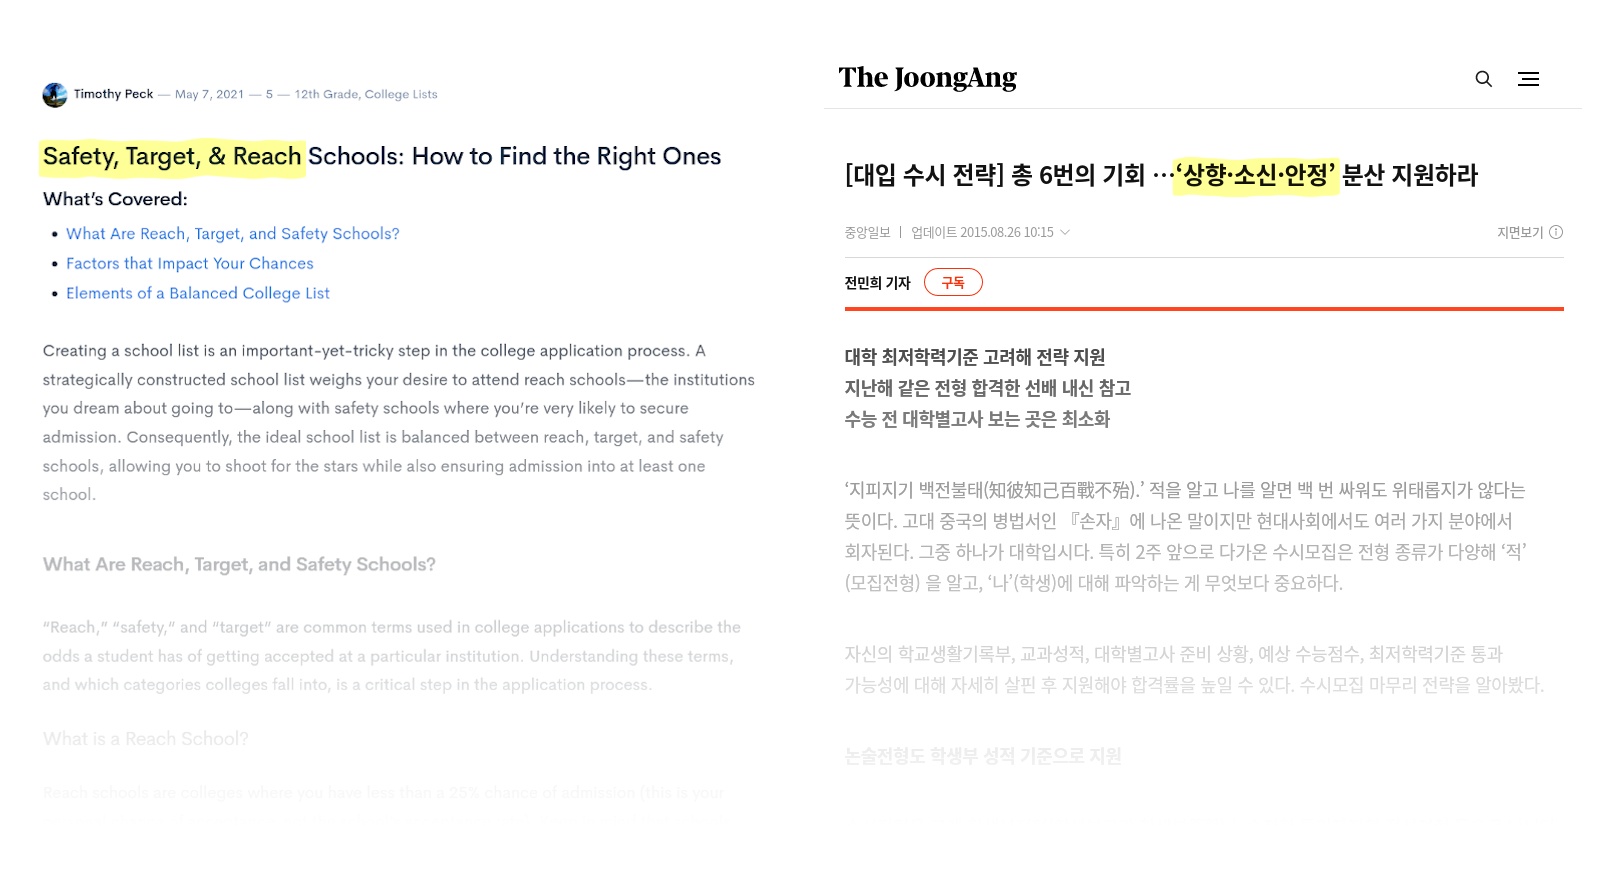
\includegraphics[width=\textwidth]{plots/news-both.png}

\ifen Do you trust the admissions consultant's advice?
\else 입학 컨설턴트의 조언, 믿을 만한가? \fi
\end{center}

\end{frame}









\ifen {
\begin{frame}{Existing solutions}
Admissions consultants recommend a \textbf{distributive heuristics} that splits applications evenly among reach, target, and safety schools. Turns out to be a \textbf{risk-averse} approach.

Another intuitive idea is the \textbf{linearization heuristic}: Since the expected utility associated with applying to $c_j$ (alone) is $f_j t_j$, solve the knapsack problem
\[\text{maximize}~~\sum_{j\in \mathcal{X}} f_j t_j \qquad \text{subject to}~~\sum_{j\in \mathcal{X}}g_j \leq H \]
as a surrogate. This solution can be \textbf{arbitrarily bad}. 

Fu (2014) solved a similar problem by \textbf{enumeration}, which is intractable for $m \geq 20$ or so.

Our algorithms provide both \textbf{time and accuracy guarantees}. 
\end{frame}
} \else {
\begin{frame}{기존의 해법}
입학 컨설팅 산업에서는 주로 ``상향·소신·안정 지원 학교'' 각각 균일하게 지원하는 \textbf{배분적 휴리스틱}을 권장하며, 이는 \textbf{위험 회피적인} 전략임을 알 수 있다. 

또한 $c_j$에만 지원할 때 기대 효용이 $f_j t_j$이므로 다음 배낭 문제를 대리 문제로 푸는 \textbf{선형화 휴리스틱}이 있다.
\[\text{maximize}~~\sum_{j\in \mathcal{X}} f_j t_j \qquad \text{subject to}~~\sum_{j\in \mathcal{X}}g_j \leq H \]
그러나 이의 \textbf{근사 계수는 $\mathbf{0}$에 무한히 가까워질 수 있다}.

Fu (2014)는 비슷한 문제를 \textbf{열거법}으로 풀었으나, $m \geq 20$일 때 비현실적인 방법이다.

본 연구는 \textbf{계산 시간과 정확도가 보장된} 알고리즘을 제시한다. 
\end{frame}
} \fi








\ifen {
\begin{frame}{Our algorithms}
In the \textbf{special case} where each $g_j = 1$, we provide an $O(m^2)$ algorithm.

The general problem is \textbf{NP-complete} (reduction from knapsack). We offer four algorithms:
\begin{itemize}
\item A linear relaxation and \textbf{branch-and-bound scheme}. Primarily of theoretical interest.

\item A \textbf{dynamic program based on total expenditures}. Exact solution in $O(Hm + m\log m)$ time (pseudopolynomial). Very fast for ``typical'' instances in which $g_j$ are small integers.

\item A different DP based on truncated portfolio valuations. $(1 - \varepsilon)$-optimal solution in $O(m^3 / \varepsilon)$ time: an \textbf{FPTAS!}
\item A \textbf{simulated annealing heuristic}. Fast, typically within 2\% of optimality.
\end{itemize}
\end{frame}
} \else {
\begin{frame}{알고리즘 제시}
모든 $g_j = 1$인 특수한 경우를 푸는 $O(m^2)$ 알고리즘 제시.

일반적인 문제는 \textbf{NP-complete} (배낭 문제에서 변환).

4개의 알고리즘 제시:
\begin{itemize}
\item 선형 완화 문제와 해당 \textbf{branch-and-bound} 해법. 일반적인 INLP 문제에 대해 자주 쓰이는 방법이다.

\item \textbf{총 지원 비용 기반 동적 계획}. (의사 다항) $O(Hm + m\log m)$ 시간에 정확한 해를 구하며, $g_j$가 작은 정수가 되는 ``전형적'' 인스턴스에 대해 매우 효율적인 해법.

\item 포트폴리오 가치의 라운딩을 이용한 동적 계획. $O(m^3 / \varepsilon)$ 시간에 $(1 - \varepsilon)$-근사해를 출력하므로 \textbf{FPTAS!}

\item \textbf{Simulated annealing} 휴리스틱. 빠르고 대부분 98\% 이상의 최적성을 얻었다.
\end{itemize}
\end{frame}
} \fi













\ifen \section{Conclusion} \else \section{결론} \fi


\ifen {
\begin{frame}{Conclusion}
``Maximax'' form, integrality constraints make the college application problem \textbf{theoretically interesting}. Formally, it is a submodular maximization problem, but its approximability is more like knapsack (cf.~Fisher et al. 1978; Kulik et al. 2013; Kellerer et al. 2004).

%The nestedness result for the $g_j = 1$ special case also resembles the knapsack problem, although the proof is more subtle. 

\looseness=-1
Solutions to the college application problem have \textbf{practical value}: US admissions consultants charge an average of \$200/hr (Sklarow 2018)!

⇒ Open-sourcing our code for public benefit (Kapur 2022).

Lots of extensions to consider: parametric risk aversion, distribution constraints, FPTAS memory-usage improvements.
\end{frame}
} \else {
\begin{frame}{결론}
\looseness=-1
``Maximax'' 형태와 정수 조건 때문에 대학 지원 문제는 \textbf{이론적으로 흥미로운 문제이다}. Submodular 최대화 문제지만, 근사 해법의 성질은 배낭 문제에 더 가깝다 (cf. Fisher et al. 1978; Kulik et al. 2013; Kellerer et al. 2004).

%$g_j=1$의 특수한 경우의 포함 사슬 관계 성질도 배낭 문제와 유사하며, 증명 과정은 좀 더 미묘하다.

좋은 대학 지원 전략에는 \textbf{금전적 가치가 있다}. 미국 입학 컨설턴트의 시간당 급료는 평균 200달러 (Sklarow 2018)!

\mbox{⇒ 공공 이익을 위해 코드는 open-source license로 공개 (Kapur 2022).}

향후 연구: 위험 회피 모수, 배분적 제약 조건 (가나다군), FPTAS의 메모리 소모량 절감.
\end{frame}
} \fi








\begin{frame}{\ifen References \else 참고 문헌 \fi}
\small
\parskip 0em
\leftskip 2em
\parindent -2em
%Balas, Egon and Eitan Zemel. 1980. ``An Algorithm for Large Zero-One Knapsack Problems.'' \emph{Operations Research} 28 (5): 1130--54. \url{https://doi.org/10.1287/opre.28.5.1130}. 

%Dantzig, George B. 1957. ``Discrete-Variable Extremum Problems.'' \emph{Operations Research} 5 (2): 266--88.

Fisher, Marshall, George Nemhauser, and Laurence Wolsey. 1978. ``An analysis of approximations for maximizing submodular set functions—I.'' \emph{Mathematical Programming} 14: 265--94.

Fu, Chao. 2014. ``Equilibrium Tuition, Applications, Admissions, and Enrollment in the College Market.'' \emph{Journal of Political Economy} 122 (2): 225--81. \url{https://doi.org/10.1086/675503}. 

Kapur, Max. 2022. ``OptimalApplication.'' GitHub repository. \url{https://github.com/maxkapur/OptimalApplication}.

%Kapur, Max and Sung-Pil Hong. 2022. ``The College Application Problem.'' Preprint. \url{https://github.com/maxkapur/CollegeApplication}.

Kellerer, Hans, Ulrich Pferschy, and David Pisinger. 2004. \emph{Knapsack Problems.} Berlin: Springer.

Kulik, Ariel, Hadas Shachnai, and Tami Tamir. 2013. ``Approximations for Monotone and Nonmonotone Submodular Maximization with Knapsack Constraints.'' \emph{Mathematics of Operations Research} 38 (4): 729--39. \url{https://doi.org/10.1287/moor.2013.0592}.

%Markowitz, Harry. 1952. ``Portfolio Selection.'' \emph{The Journal of Finance} 7 (1): 77--91. \url{https://www.jstor.org/stable/2975974}.
%
%Rozanov, Mark and Arie Tamir. 2020. ``The nestedness property of the convex ordered median location problem on a tree.'' \emph{Discrete Optimization} 36: 100581. \url{https://doi.org/10.1016/j.disopt.2020.100581}.

Sklarow, Mark. 2018. \emph{State of the Profession 2018: The 10 Trends Reshaping Independent Educational Consulting.} Technical report, Independent Educational Consultants Association. \url{https://www.iecaonline.com/wp-content/uploads/2020/02/IECA-Current-Trends-2018.pdf}.

\end{frame}















\end{document}







\ifen \section{Appendix} \else \section{부록} \fi

\begin{frame}{\ifen Appendix: Summary of algorithms\else 부록: 알고리즘 요약\fi}
\begin{center}
\ifen
\scalebox{0.90}{ 
\begin{tabular}{r|lllll}
\textbf{Algorithm} & \textbf{Problem} & \textbf{Restrictions} & \textbf{Exactness}       & \textbf{Computation time} \\ \hline
\xrowht[()]{1.5em}  \begin{tabular}[r]{@{}r@{}}Na\"ive\end{tabular} &  \begin{tabular}[l]{@{}l@{}}Homogeneous \\ costs\end{tabular}     & None                  & $(1/h)$-opt.               & $O(m)$                    \\ 
\xrowht[()]{1.5em}  Greedy                &   \begin{tabular}[l]{@{}l@{}}Homogeneous \\ costs\end{tabular}    & None                  & Exact                    & $O(hm)$                   \\
\xrowht[()]{1.5em}  \begin{tabular}[r]{@{}r@{}}Branch and\\ bound\end{tabular}   & General          & None                  & Exact                    & $O(2^m)$                  \\
\xrowht[()]{1.5em}  Costs DP     &   General          & $g_j$ integer         & Exact                    & $O(Hm + m \log m)$        \\
\xrowht[()]{1.5em}  FPTAS      &   General          & None        & $(1 - \varepsilon)$-opt. & $O(m^3 / \varepsilon)$   \\
\xrowht[()]{1.5em}  \begin{tabular}[r]{@{}r@{}}Simulated\\annealing\end{tabular}   & General          & None                  & $0$-opt.                    & $O(Nm)$                
\end{tabular}
}
\else
\scalebox{1}{ 
\begin{tabular}{r|lllll}
\textbf{알고리즘} &  \textbf{문제} & \textbf{제한} & \textbf{정확도}       & \textbf{계산 시간} \\ \hline
\xrowht[()]{1.7em}  \begin{tabular}[r]{@{}r@{}}나이브\end{tabular}                & \begin{tabular}[l]{@{}l@{}}동일한\\ 지원 비용\end{tabular}     & 없음                  & $(1/h)$-근사          & $O(m)$                    \\ 
\xrowht[()]{1.7em}  탐욕 해법               &  \begin{tabular}[l]{@{}l@{}}동일한\\ 지원 비용\end{tabular}    & 없음                  & 정확                    & $O(hm)$                   \\
\xrowht[()]{1.7em}  \begin{tabular}[r]{@{}r@{}}분지한계법\end{tabular}   & 일반 문제          & 없음                  & 정확                    & $O(2^m)$                  \\
\xrowht[()]{1.7em}   \begin{tabular}[r]{@{}r@{}}지출액\\ 동적 계획\end{tabular}    & 일반 문제          & $g_j$ 정수         & 정확                    & $O(Hm + m \log m)$        \\
\xrowht[()]{1.7em}  FPTAS       & 일반 문제          & 없음        & $(1 - \varepsilon)$-근사 & $O(m^3 / \varepsilon)$   \\
\xrowht[()]{1.7em}   \begin{tabular}[r]{@{}r@{}}모의\\ 담금질\end{tabular}    & 일반 문제          & 없음                      & $0$-근사                    & $O(Nm)$                
\end{tabular}
}
\fi
\end{center}
\end{frame}
